
\begin{figure}[ht!]\centering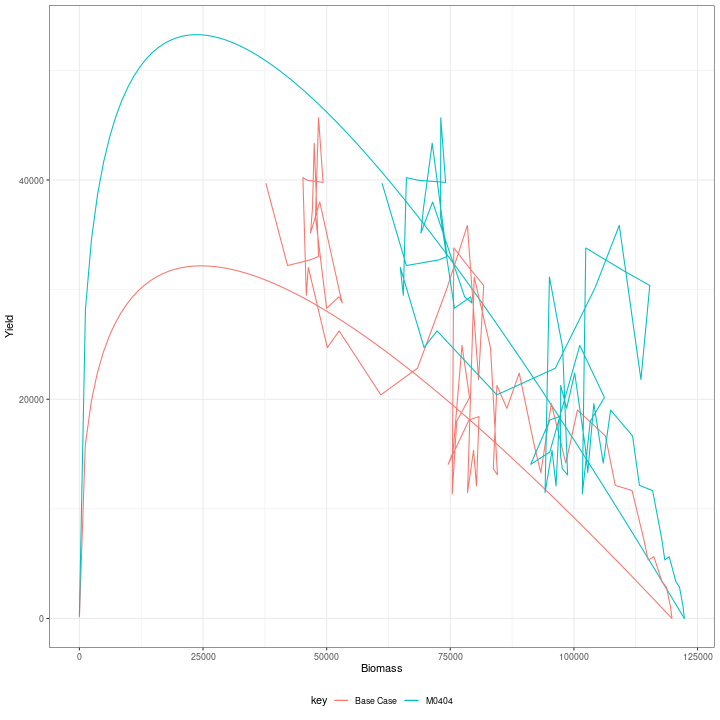
\includegraphics[width=0.75\textwidth]{figures/pf-2-1.png} \caption{Production function for base case and MMat=0.4.}
\label{fig:pf2}       
\end{figure}

\begin{figure}[ht!]\centering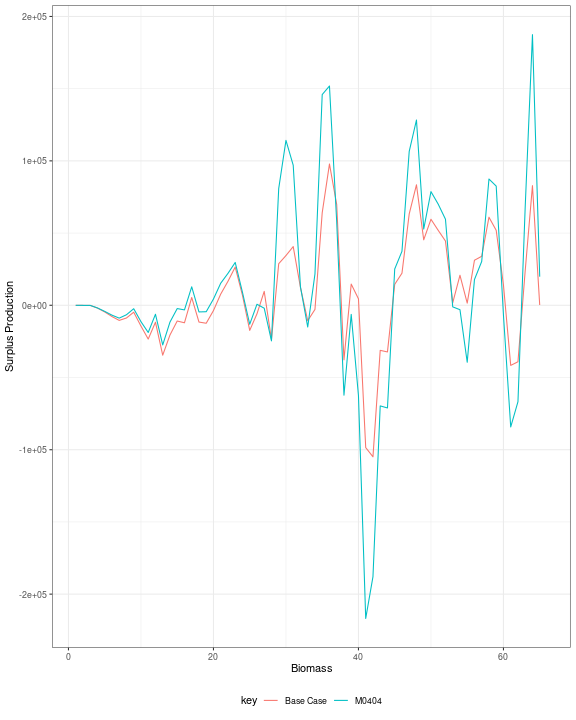
\includegraphics[width=0.75\textwidth]{figures/sp-y-2-1.png} \caption{Process error for base case and MMat=0.4.}
\label{fig:pe2}       
\end{figure}

\begin{figure}[ht!]\centering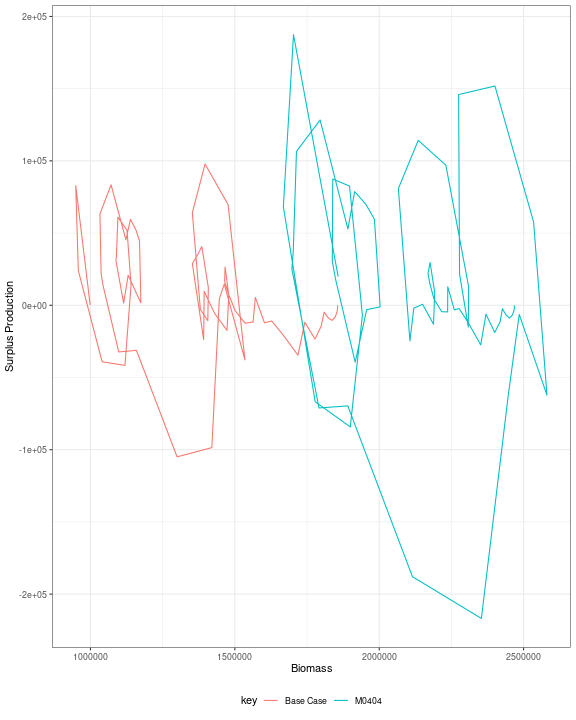
\includegraphics[width=0.75\textwidth]{figures/sp-b-2-1.png} \caption{Surplus production for base case and MMat=0.4.}
\label{fig:sp2}       
\end{figure}

\begin{figure}[ht!]\centering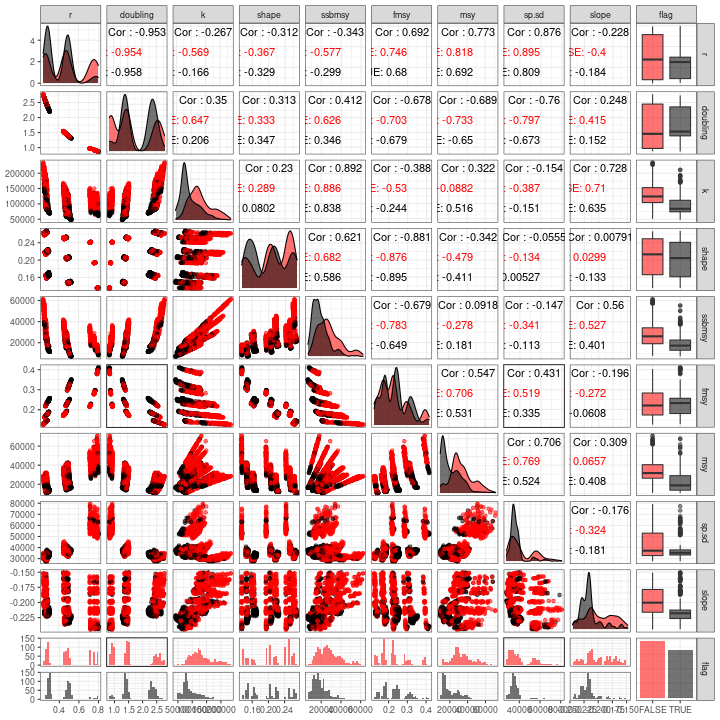
\includegraphics[width=0.75\textwidth]{figures/param-pairs-mohn3-1.png} \caption{Summary of estimated stock dynamics quantities, contrasting those that pass the Mohn's $\rho$ test with those that fail.}
\label{fig:param-pairs-1}       
\end{figure}

\begin{figure}[ht!]\centering\includegraphics[width=0.75\textwidth]{figures/main-retro-1.png}  
\caption{Retrospective analysis of spawning stock biomass for the main effects of the Indian Ocean albacore assessment model grid. The black thick line shows the estimated CPUE index by the reference model fitted to all years with observations and cyan lines show the respective CPUE fits with red points denoting the last years of the retrospective 'peels'.}
\label{fig:retro}      
\end{figure}

\begin{figure}[ht!]\centering\includegraphics[width=0.75\textwidth]{figures/mohn-1.png}  \caption{Summary of Mohn's $\rho$ for the for the 1440 assessment models in the Indian Ocean albacore tuna grid, with main effects indicated by the vertical lines.} 
\label{fig:mohn}       
\end{figure}


\begin{figure}[ht!]\centering\includegraphics[width=0.75\textwidth]{figures/kobe-main-mohn-1.png} 
\caption{Kobe phase plot showing spawning biomass ($B$) and fishing mortality ($F$) relative to $MSY$ target reference points in the terminal year for the 13 main effect models, identifying those scenarios that pass and fail the Mohn's $\rho$ test. Within model uncertainty was approximating using multivariate log-normal distribution derived from Hessian matrix (MVLN) with cyan points denoting the medians. } 
\label{fig:kb-mohn}    
\end{figure}

\begin{figure}[ht!]\centering\includegraphics[width=0.75\textwidth]{figures/kobe-mohn-1.png} \caption{Kobe phase plot showing spawning biomass ($B$) and fishing mortality ($F$) relative to $MSY$ target reference points in the terminal year for 1440 grid models, identifying those that pass the Mohn's $\rho$ test.}
\label{fig:kobe}       
\end{figure}

\begin{figure}[ht!]\centering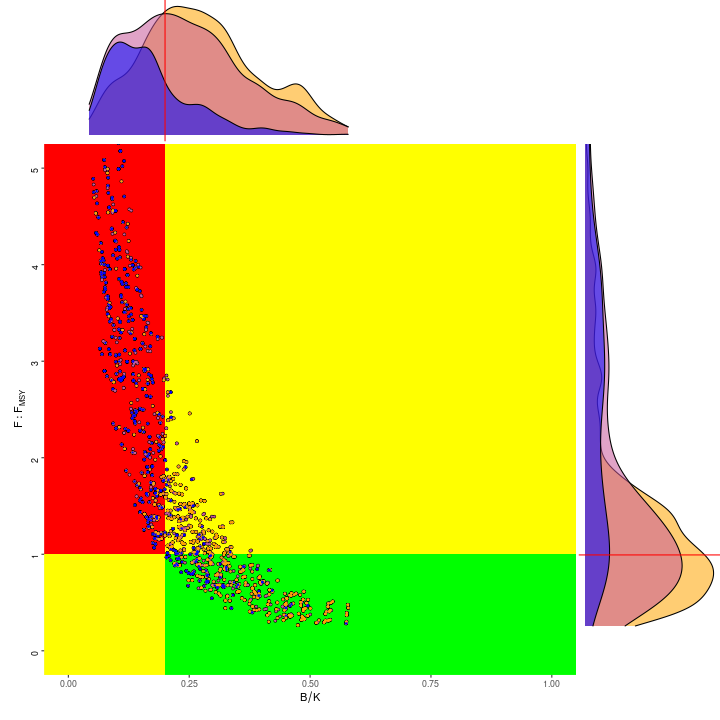
\includegraphics[width=0.75\textwidth]{figures/majuro-mohn-1.png}    
\caption{Majuro phase plot showing spawning biomass ($B$) relative to the unfished state ($K$) and fishing mortality ($F$) relative to the $MSY$ target reference points in the terminal year, for all 1440 grid models, identifying those that pass the Mohn's $\rho$ test.}
\label{fig:majuro}     
\end{figure}

\begin{figure}[ht!]\centering\includegraphics[width=0.75\textwidth]{figures/retro3-1.png}  
\caption{Retrospective analysis with three year projection of spawning stock biomass for the main effects of the Indian Ocean albacore assessment model grid. The black thick line shows the estimated CPUE index by the reference model fitted to all years with observations and cyan lines show the respective CPUE fits with red points denoting the last years of the retrospective 'peels'.}
\label{fig:retro3}      
\end{figure}

\begin{figure}[ht!]\centering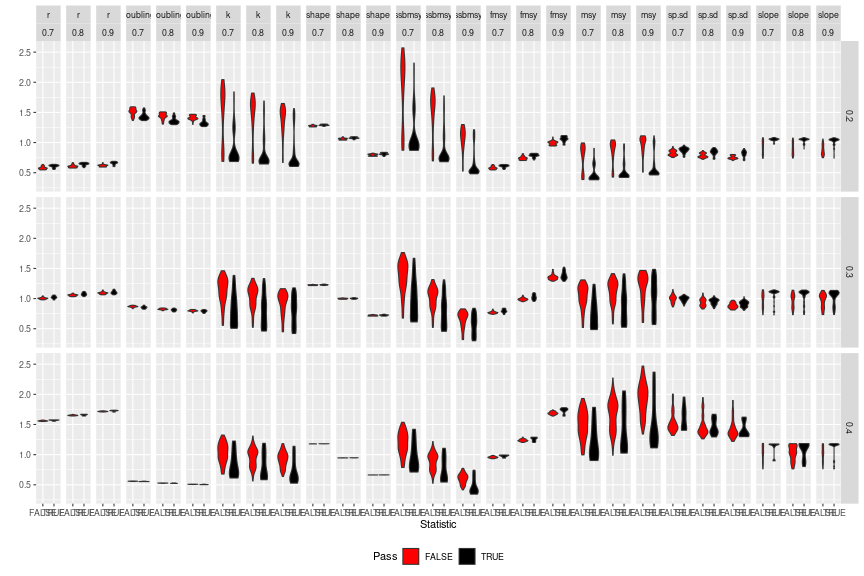
\includegraphics[width=0.75\textwidth]{figures/param-box-mohn-1.png} \caption{Boxplots showed estimated stock dynamics quantities, contrasting the effect size of those that pass the Mohn's $\rho$ test with those that fail.}
\label{fig:param-box-1}       
\end{figure}

\begin{figure}[ht!]\centering\includegraphics[width=0.75\textwidth]{figures/param-pairs-mohn-1.png} \caption{Summary of estimated stock dynamics quantities, contrasting those that pass the Mohn's $\rho$ test with those that fail.}
\label{fig:param-pairs3-1}       
\end{figure}

\begin{figure}[ht!]\centering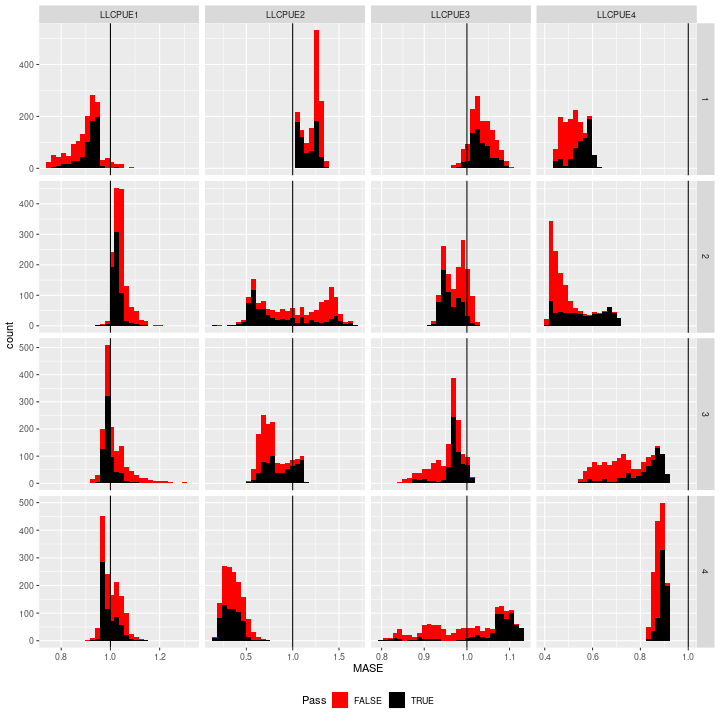
\includegraphics[width=0.75\textwidth]{figures/mase-1.png} \caption{Summary of MASE.}
\label{fig:wts}       
\end{figure}

\begin{figure}[ht!]\centering\includegraphics[width=0.75\textwidth]{figures/pf-b-1.png} \caption{Production functions with yield v biomass for main effects.}
\label{fig:sp-main}       
\end{figure}

\begin{figure}[ht!]\centering\includegraphics[width=0.75\textwidth]{figures/sp-b-1.png} \caption{Surplus production v biomass for main effects.}
\label{fig:sp-main}       
\end{figure}

\begin{figure}[ht!]\centering\includegraphics[width=0.75\textwidth]{figures/pf-b-1.png} \caption{Surplus production v biomass  for main effects.}
\label{fig:sp-main}       
\end{figure}
